\chapter{Proposta}

Este capítulo tem como objetivo apresentar a proposta de intervenção na plataforma Brasil Participativo, esclarecendo os detalhes relevantes sobre as estratégias de otimização que podem vir a serem adotadas. A Seção \ref{sec:contextualizando_a_plataforma_brasil_participativo} explica o que é a plataforma, sobre como ela nasceu, seus objetivos futuros e os já alcançados. A Seção \ref{sec:aspectos_tecnicos_da_plataforma_brasil_participativo} aborda os aspectos técnicos da plataforma em nível de código-fonte e arquitetura, revelando o funcionamento das principais partes e o uso do \textit{framework Ruby on Rails}. Na Seção \ref{sec:principais_problemas_de_performance_da_plataforma_brasil_participativo}, são expostos os desafios enfrentados pela plataforma no ano de 2023, explorando as possibilidades de intervenção para otimização. A Seção \ref{sec:proposta_de_intervencao_na_plataforma_brasil_participativo} tem como objetivo listar potenciais intervenções para melhorar a performance, esclarecendo a abordagem a ser adotada e o grau de esforço envolvido.

\section{Contextualizando a Plataforma Brasil Participativo}
\label{sec:contextualizando_a_plataforma_brasil_participativo}

A Plataforma Brasil Participativo é uma iniciativa do governo federal voltada para a promoção da participação social. Desenvolvida em software livre com o apoio de diversos parceiros, incluindo a Dataprev, a comunidade Decidim-Brasil, o Ministério da Gestão e Inovação em Serviços Públicos (MGI) e a Universidade de Brasília (UnB), ela foi criada sob a responsabilidade da Secretaria Nacional de Participação Social da Secretaria Geral da Presidência da República (SNPS/SGPR).

A plataforma tem como propósito possibilitar que a população contribua ativamente na criação e melhoria das políticas públicas. Uma de suas primeiras iniciativas foi o Plano Plurianual Participativo, assinado pela SGPR e pelo Ministério do Planejamento e Orçamento (MPO). Durante o período de 11 de maio a 16 de julho de 2023, a plataforma permitiu a coleta de propostas da sociedade e a priorização de programas e propostas para o Plano Plurianual (PPA) 2024-2027.

A participação ativa na etapa digital do PPA atingiu mais de um milhão e quatrocentas mil pessoas (1.400.000), conquistando o título de maior experiência de participação social na internet realizada pelo governo federal. A plataforma continuará evoluindo, permitindo que conselhos nacionais criem suas páginas, ministérios realizem consultas públicas e órgãos federais promovam a participação da população na definição de decretos, portarias e outras ações.

Essa abertura à participação digital representa um marco importante para a democracia, possibilitando que cidadãos influenciem diretamente nas decisões governamentais. A Plataforma Brasil Participativo oferece a oportunidade de criação de perfis individuais para facilitar a participação ativa dos interessados \cite{brasilparticipativo-sobre}.

\section{Aspectos Técnicos da Plataforma Brasil Participativo}
\label{sec:aspectos_tecnicos_da_plataforma_brasil_participativo}

Nesta seção será abordada a maneira como foi desenvolvida a plataforma Brasil Participativo utilizando-se do \textit{framework Ruby on Rails} e da \textit{gem Decidim}. O objetivo dessa seção é elucidar como a plataforma foi inicialmente desenvolvida, o atual estado, e explorar em detalhes a \textit{gem Decidim}.

\subsection{Como foi Desenvolvida a Plataforma Brasil Participativo}

A plataforma Brasil Participativo foi desenvolvida com o \textit{framework Ruby on Rails} utilizando a \textit{gem Decidim}. Segundo a própria documentação disponibilizada pela comunidade de contribuidores do \textit{Decidim}, a \textit{gem} é descrita como um \textit{framework} que visa possibilitar que qualquer pessoa possa criar uma plataforma \textit{web} para ser utilizada como rede política para participação democrática. O Decidim fornece a organizações a capacidade de criar processos para planeamento estratégico, orçamento participativo, concepção colaborativa de regulamentos, espaços urbanos e processos eleitorais \cite{decidim-about}.

A plataforma no presente momento se apoia totalmente nas funcionalidades disponibilizadas pela \textit{gem Decidim}, preocupando-se apenas em implementar em sua instância correções de \textit{bugs}, customizações de estilo e comportamento de regras de negócio, e funcionalidades extras. De fato, a maior parte do código executado na plataforma não é visto em seu repositório oficial, pois este está abstraído dentro da \textit{gem Decidim}. O repositório oficial do Brasil Participativo está disponível no \textit{Gitlab} no endereço: \href{https://gitlab.com/lappis-unb/decidimbr/decidim-govbr}{https://gitlab.com/lappis-unb/decidimbr/decidim-govbr}. Já o repositório oficial do \textit{Decidim} está disponível no \textit{Github} no endereço: \href{https://github.com/decidim/decidim}{https://github.com/decidim/decidim}.


\subsection{Arquitetura do Decidim}

O Decidim possui várias entidades em sua arquitetura, mas as mais importantes para entendimento da regra de negócio são os espaços participativos e os componentes, referidos na documentação como \textit{participatory spaces} e \textit{components}, respectivamente. Uma visão macro das entidades do \textit{Decidim} pode ser visto na Figura \ref{fig:arquitetura-decidim}. O \textit{Decidim} armazena dados de cada uma dessas estruturas utilizando a abordagem padrão de aplicações \textit{Rails like}, isto é, utilizando-se do \textit{Active Record} e persistindo os dados em um banco de dados relacional, o \textit{PostgreSQL}.

\begin{figure}[htbp]
  \centering
  \caption{Arquitetura do \textit{Decidim}}
  \label{fig:arquitetura-decidim}
  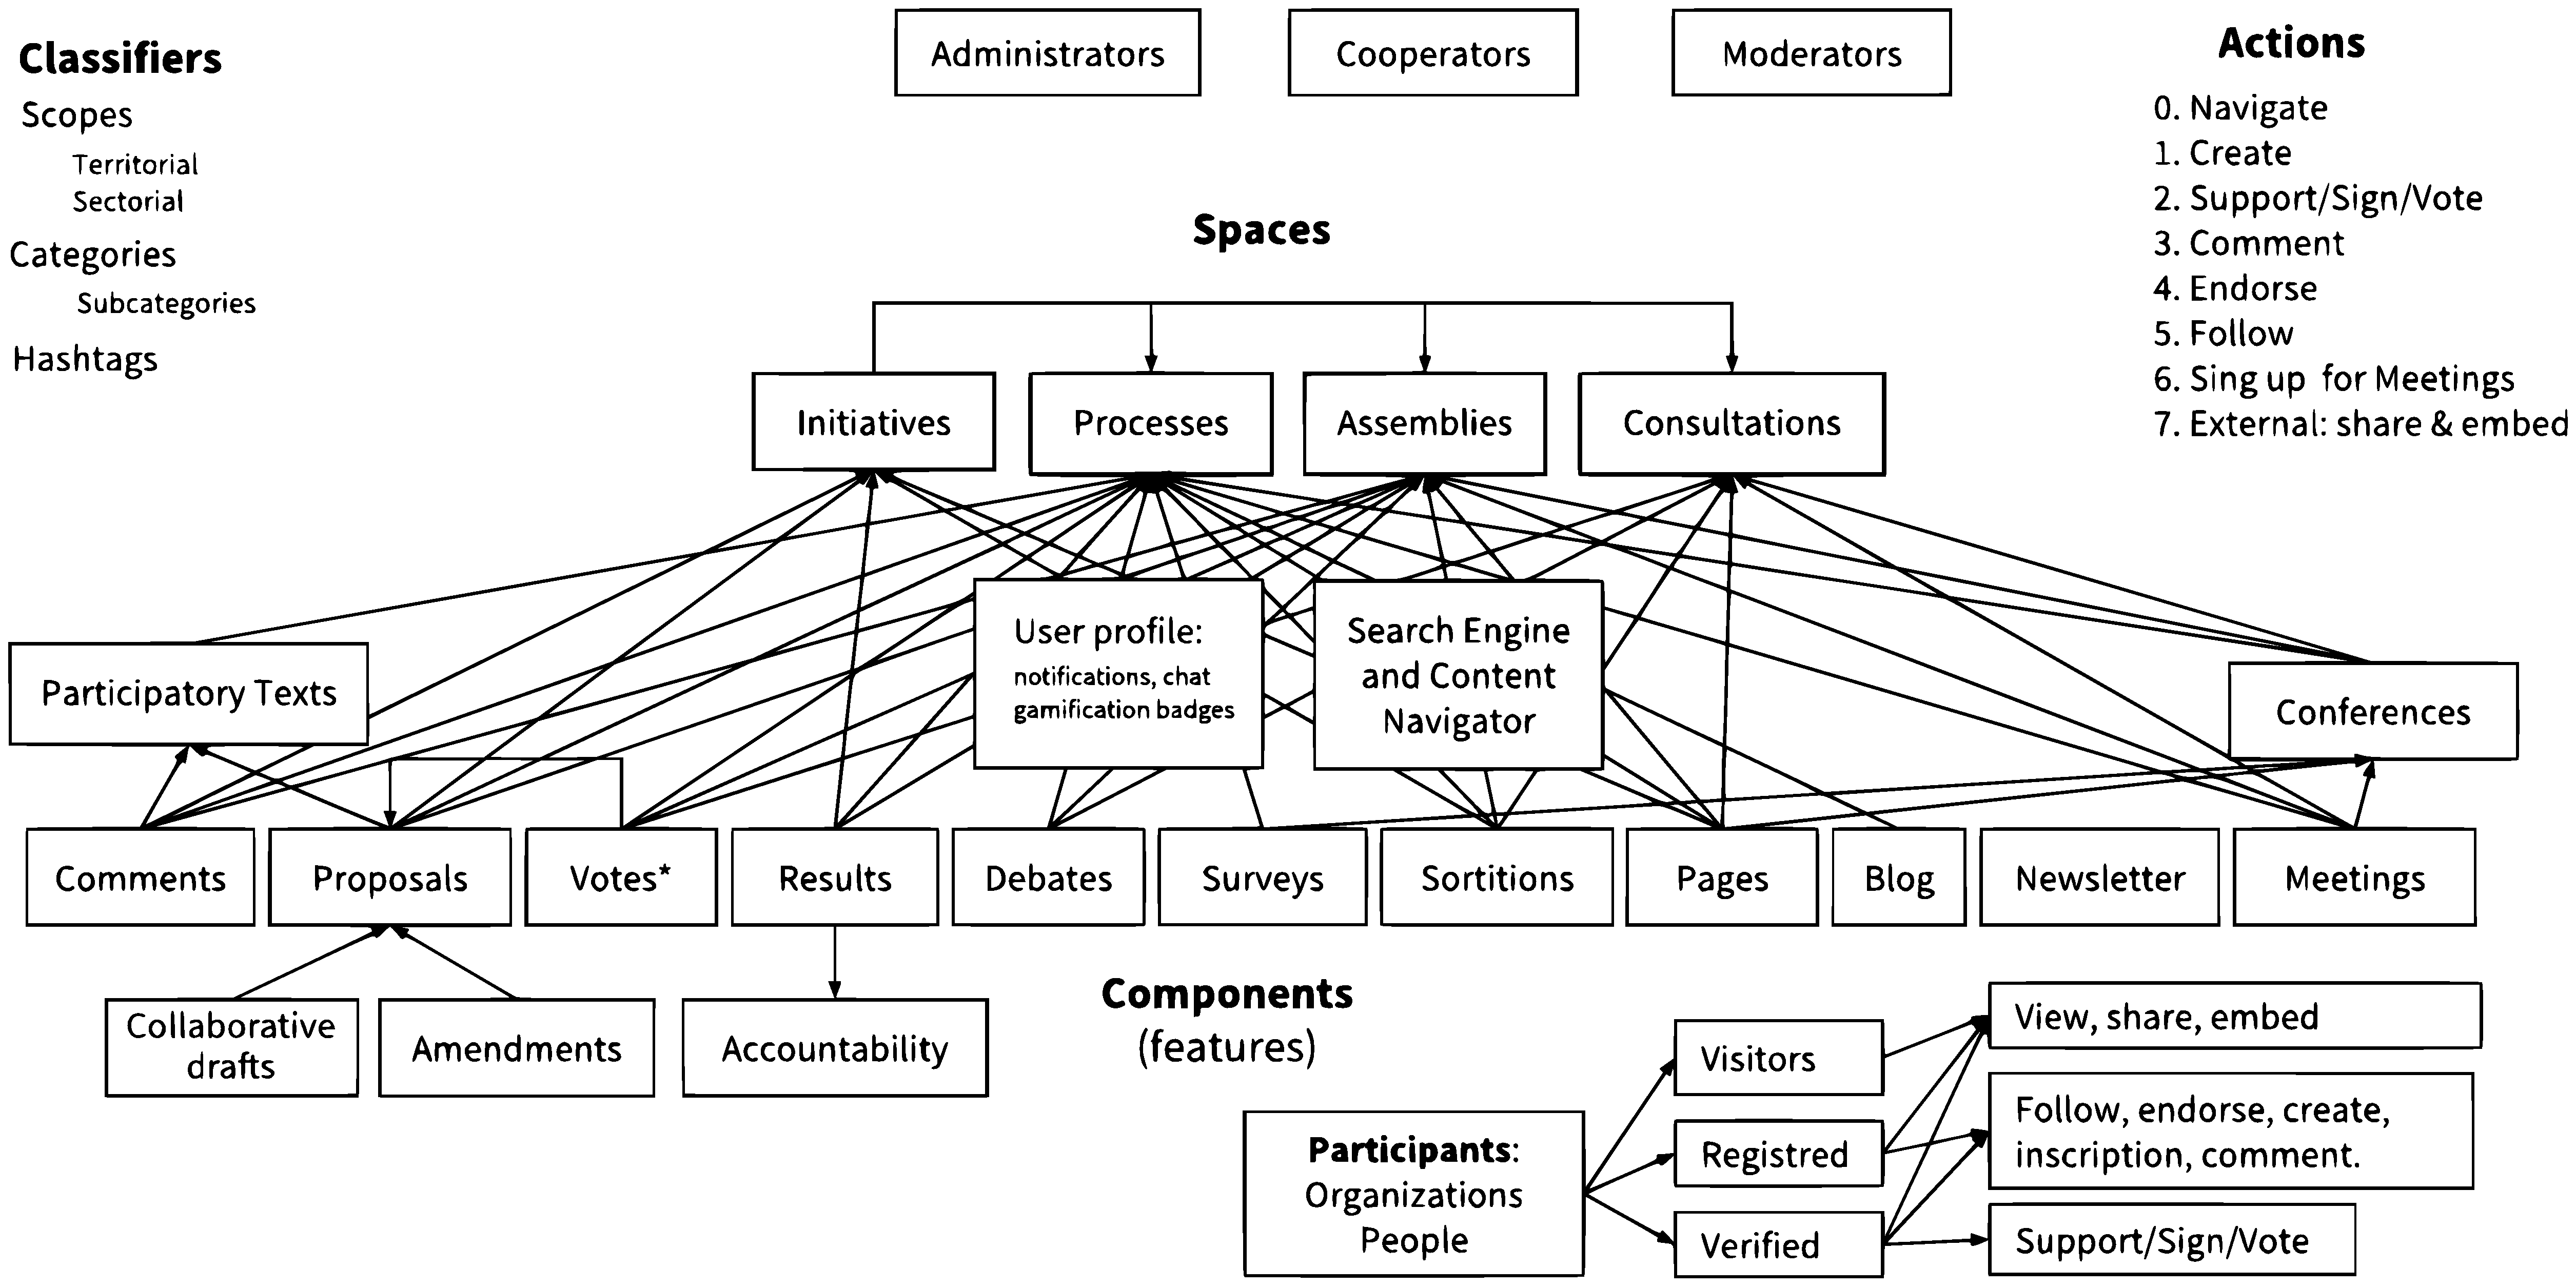
\includegraphics[width=\textwidth]{figuras/diagrama_decidim-min.eps}
  \fonte{\cite{decidim-descriptionpage}}
\end{figure}

\subsubsection{Participatory Spaces}

Os \textit{participatory spaces} são \textit{frameworks} que definem como a participação será realizada, os canais ou meios pelos quais cidadãos ou membros de uma organização podem processar solicitações ou coordenar propostas e tomar decisões. Iniciativas, processos, assembleias e consultas são todos espaços participativos, estes referidos na documentação como \textit{initiatives}, \textit{participatory processes}, \textit{assemblies} e \textit{consultations}, respectivamente. Exemplos específicos incluem: uma iniciativa cidadã para alterar diretamente uma regulamentação; uma assembleia geral ou conselho de trabalhadores; um orçamento participativo, planejamento estratégico ou processo eleitoral; um referendo ou uma convocação para votar "Sim" ou "Não" para mudar o nome de uma organização \cite{decidim-descriptionpage}.

A nível de código, cada implementação de um novo \textit{participatory space} é feita em um sub-modulo separado em uma \textit{gem} própria. Uma relação entre cada um dos espaços participativos já existentes por padrão no \textit{Decidim} e o seu respectivo sub-modulo pode ser vista no Quadro \ref{tab:modulos-participatoryspaces}.

\begin{table}
  \centering
  \caption{Módulos dos espaços participativos padrões do \textit{Decidim}}
  \label{tab:modulos-participatoryspaces}
  \begin{tabular}{|c|c|c|}
    \hline
    Espaço Participativo & Módulo \\
    \hline
    Assembleias & decidim-assemblies \\
    Consultas ou Eleição & decidim-elections \\
    Iniciativas & decidim-initiatives \\
    Processos Participativos & decidim-participatory\_processes \\
    \hline
  \end{tabular}
  \fonte{\cite{decidim-descriptionpage}}
\end{table}

\subsubsection{Components}

Os \textit{components} são os mecanismos participativos que permitem uma série de operações e interações entre os usuários da plataforma dentro de cada um dos espaços participativos. No \textit{Decidim} há disponível por exemplo os seguintes componentes: comentários, propostas, debates, pesquisas, sorteios, blogs e reuniões. Outros componentes que se baseiam nos componentes básicos são: textos participativos, responsabilidade e conferências \cite{decidim-descriptionpage}.

Da mesma forma que ocorre com os espaços participativos, os componentes são implementados através de sub-módulos em formato de novas \textit{gems}. No Quadro \ref{tab:modulos-components} é possível conferir o nome do módulo de cada componente fornecido por padrão pelo \textit{Decidim}.

\begin{table}
  \centering
  \caption{Módulos dos componentes padrões do \textit{Decidim}}
  \label{tab:modulos-components}
  \begin{tabular}{|c|c|c|}
    \hline
    Componente & Módulo \\
    \hline
    Comentários & decidim-comments \\
    Propostas & decidim-proposals \\
    Debates & decidim-debates \\
    Pesquisas & decidim-surveys \\
    Sorteios & decidim-sortitions \\
    \textit{Blogs} & decidim-blogs \\
    Reuniões & decidim-meetings \\
    \hline
  \end{tabular}
  \fonte{\cite{decidim-descriptionpage}}
\end{table}

\section{Principais Problemas de Performance da Plataforma Brasil Participativo}
\label{sec:principais_problemas_de_performance_da_plataforma_brasil_participativo}

No ano de 2023 o Brasil Participativo acumulou um milhão e quatrocentos mil usuários únicos. Tal volume de usuários implicou que a plataforma exibisse problemas de performance que foi observado pelos usuários através da indisponibilidade do serviço durante o período de alta demanda. Conforme apontado pela Dataprev, empresa responsável pela infraestrutura da aplicação no ambiente produtivo, muitos problemas de diferentes naturezas foram notados: sobreutilização do banco de dados e a indisponibilidade do mesmo, falta do uso de índices e \textit{memory leak}.

\subsection{Sobreutilização do Banco de Dados e Indisponibilidade}

Foi notado pela Dataprev que o acesso a páginas de propostas e criação de novos usuários gera enorme utilização do banco de dados. Um dos problemas mais óbvios capturado foi a utilização do comando SQL \textit{ILIKE} para desambiguação de \textit{nicknames} na plataforma. Comando este que requer bastante processamento do banco de dados, atingindo tempos na casa de dois segundos. Requisições que demandam tanto tempo do banco de dados, aliadas à alta demanda de usuários, fizeram com que o PostgreSQL atingisse o limite de conexões em seu \textit{pool} em vários momentos. No ambiente produtivo, o tempo de espera limite para obtenção de uma conexão do \textit{pool} do banco de dados é de cinco segundos, porém diversas requisições retornaram com erro para os usuários por exceder esse tempo limite. Desta forma, conclui-se que muitas ações do sistema utilizam de forma excessiva o banco de dados, sendo necessária uma estratégia de refatoração para que este problema seja resolvido.

\subsection{Ausência do Uso de Índices em Consultas Ofensoras na Plataforma}

Foi constatado pela Dataprev que as sete principais consultas mais ofensoras da plataforma poderiam ter seu desempenho melhorado através do uso de índices em suas tabelas no banco de dados. Através da observação do uso da plataforma no ano de 2023, um padrão de consultas recorrentes foi observado. A Dataprev iniciou um trabalho interno para implementação dos índices no banco de dados. A criação desses índices pode ser proposta para a comunidade Decidim posteriormente, com o intuito de torná-la padrão no projeto.

\subsection{Memory Leak do processo Ruby}

A Dataprev observou que, com o tempo, a memória alocada para a execução da aplicação \textit{Rails} aumenta sem dar qualquer indícios de recuo, o que implicou em um trabalho extra por parte da equipe para reiniciar a aplicação sempre que esta atingisse um determinado teto de uso de memória.

\section{Proposta de Intervenção na Plataforma Brasil Participativo}
\label{sec:proposta_de_intervencao_na_plataforma_brasil_participativo}

Dentre os vários problemas citados, aqueles que mais impactam no uso da plataforma são os relacionados com o uso excessivo do banco de dados PostgreSQL. Muitas requisições geram dezenas de chamadas ao banco de dados para poder fornecer informações aos usuários em tempo real. Sendo assim, a proposta de intervenção fornecida neste trabalho assumirá a seguinte premissa:

\begin{itemize}
    \item Toda informação dentro da plataforma possui um grau de tolerância para o atraso da disponibilização do seu estado atual para uma determinada funcionalidade.
\end{itemize}

Isto é, uma determinada informação poderá ser exibida de forma desatualizada por um determinado tempo em uma funcionalidade específica, gerando pouco ou nenhum prejuízo à experiência de uso do usuário, e à análise dos dados na plataforma. Também é assumido que, nem em toda funcionalidade da plataforma será aceitável a utilização de \textit{cache}. Enquanto em páginas públicas ter dados desatualizados por segundos ou minutos pode ser visto como aceitável, o mesmo pode não ser verdade para funcionalidades que gerem relatórios utilizados pela administração da plataforma. Dessa forma, o foco principal neste trabalho, se concentrará no estudo e na aplicação das estratégias de uso das tecnologias de armazenamento de \textit{cache} para que estas sejam aplicadas na arquitetura da aplicação, de tal forma que hajam melhorias de performance observáveis.

\subsection{Abordagem}

A abordagem se constituirá das seguintes atividades:

\begin{enumerate}
    \item Coleta das requisições mais comuns, e com maior impacto, na plataforma através da análise da Dataprev;\label{enum:coleta_das_requisicoes}
    \item Análise das requisições, com objetivo de entender quais funcionalidades da aplicação são utilizadas, e quais possuem maior impacto no \textit{response time};
    \item Análise da aceitação das funcionalidades em relação ao uso de \textit{cache};
    \item Desenvolvimento da alteração;
    \item Testes de performance.
\end{enumerate}

\subsubsection{Coleta das requisições mais comuns}

A Dataprev disponibilizou no segundo semestre de 2023 uma planilha com os problemas anteriormente citados, e em reunião, exibiu exemplos de requisições frequentes que possuem grande impacto no sistema. Agora, será solicitado um relatório completo das requisições realizadas na plataforma, com o máximo de detalhes que for possível sobre: a frequência com que a requisição ocorre, a quantidade de consultas realizadas no banco, o tempo total utilizado pelo banco de dados para buscar as informações necessárias, o tempo total utilizado pela aplicação \textit{Rails} para renderizar as informações sobre os \textit{templates} utilizados, e o \textit{response time} da requisição. Destas requisições, serão priorizadas as mais frequentes e com maior \textit{response time}.

\subsubsection{Análise das requisições}

No conjunto das requisições escolhidas, cada uma delas será analisada a fim de descobrir as funcionalidades e mecanismos da aplicação envolvidos em sua execução. O \textit{Decidim} implementa diversos módulos e \textit{mixins} que são reaproveitados ao longo da aplicação, sendo assim, o objetivo dessa atividade é mapear quais destas funcionalidades possuem maior impacto na performance.

\subsubsection{Análise da Aceitação sobre o Uso do Cache}

Como mencionado, presume-se que a plataforma possui um grau de tolerância sobre a exibição de dados desatualizados em certas páginas. Dessa maneira, cada funcionalidade será avaliada de tal forma que sejam identificadas brechas para inserção do uso de estratégias de \textit{cache}. Nesse momento, é esperado que nem todas funcionalidades aceitem a inserção de \textit{cache} diretamente no núcleo de sua estrutura, sendo assim, cada cliente de cada funcionalidade será avaliado separadamente para estudar a possibilidade de adoção de \textit{cache}. O cliente de uma funcionalidade pode ser uma \textit{model}, uma \textit{controller} ou uma \textit{view}.

\subsubsection{Desenvolvimento da alteração}

Após mapeados os pontos passíveis de utilização de \textit{cache} na aplicação, será desenvolvida a especificação funcional da alteração, deixando explícito quais pontos foram alterados, quais estratégias foram adotadas, e os impactos previstos sobre o estado dos dados exibidos para o usuário.

\subsubsection{Testes de performance}

Para cada funcionalidade alterada, serão realizados testes de performance sobre as requisições que a utilizam, buscando aferir o ganho de performance, se houver, depois da adoção da estratégia de armazenamento em cache. Serão executadas baterias de testes nas requisições escolhidas na atividade \ref{enum:coleta_das_requisicoes} utilizando a infraestrutura disponibilizada pelo laboratório Lappis. Para execução dos testes, será utilizado a ferramenta \textit{ApacheBench} que permite a simulação de diversas requisições compilando dados de \textit{response time} e \textit{throughput} da aplicação.

\subsection{Cronograma}

Para cumprimento das atividades listadas, foi elaborado um cronograma que pode ser conferido no Quadro \ref{tab:cronograma-tcc2}. Atividades de maior complexidade foram dividas em atividades menores para melhor gerenciamento de calendário.

\begin{table}
  \centering
  \caption{Cronograma de Atividades de Desenvolvimento}
  \label{tab:cronograma-tcc2}
  \begin{tabular}{|c|c|}
    \hline
    Data de inicio & Atividade \\
    \hline
    15/01/2024 & Solicitação do relatório para Dataprev \\
    01/02/2024 & Análise do relatório disponibilizado \\
    12/02/2024 & Escolha das requisições mais coerentes para o escopo do trabalho \\
    19/02/2024 & Análise das principais funcionalidades ou módulos utilizados \\
    01/03/2024 & Estudo e implementação das estratégias de cache \\
    01/04/2024 & Finalização da implementação e criação da especificação técnica \\
    01/05/2024 & Testes finais e compilação dos resultados \\
    \hline
  \end{tabular}
\end{table}

\section{Considerações Finais do Capítulo}

Neste capítulo, foram explorados detalhes cruciais sobre a arquitetura da plataforma Brasil Participativo, destacando a utilização da tecnologia \textit{Ruby on Rails} e da \textit{gem Decidim}. Compreender a arquitetura é fundamental para otimizar o desempenho da aplicação e proporcionar uma experiência aprimorada aos usuários. Para aprimorar a performance da plataforma, foi traçado um plano de ações consistente que envolverá pesquisa, desenvolvimento e testes. A execução dessas atividades visam não apenas a melhoria do desempenho da aplicação, mas também a garantia de uma experiência mais satisfatória para os usuários da plataforma Brasil Participativo, possibilitando maior facilidade na participação digital.